\clearpage
\begin{flushright}
	\textit{Лекция №13}
	\textit{2016.05.30}
\end{flushright}

Демон $ksoftirqd$ – поток ядра, на каждый процесоор по одному потоку в системе, его можно увидеть в системе и он имеет соответствующий номер (ядра).

Есть аппаратные прерывания, высокоприоритетные, и это прерывание ставит отложенное прерывание (в данном случае $SOFTIRQ$ или $тасклет$ в очередь на выполнение) и такое поставленное в очередь отложенное действие будет выполнено. Часто, отложенные прерывания $SOFTIRQ$ могут сами себя вызывать. Это характерно для сетевой карты. Когда с высокой частотой на вход поступают пакеты. В результате процессор не успевают закончить обработку одно прерывания, а уже пришло следующее. Тогда система ставит эти действия в очередь (создает очередь для их последующей обработки) с помощью процесса $ksoftirqd$. Эти действия выполняются в фоновом режиме, потому что имеется следующая ситуация: если обрабатывать отложенные действия по их возникновению, может возникнуть ситуация, когда процессору не хватит времени для обработки приложений. Если прерывание само себя запускает, то эти действия обрабытваются в контексте процесса и фактически они имеют nice = 19 (почти фоновое выполнение, они выполняются, но не сразу). Если этот демон занимает больше, чем какой то процент процессорного времени то считается, что система находится под сильной нагрузкой прерываний.

Если $softinterrapt$   срабатывает во второй раз и в это время обрабатываются какие то софтинтерапты, то запускается демон $ksoftirqd$  чтобы обработать этот запустивший себя второй раз $SOFTIRQ$ в контексте процесса, практически в фоне. Таким образом достигается баланс. Софтинтеррапт обрабатывают сетевую карту. 

Драйвер предназначен для управления внешним устройством, подключаем к компьютеру. Есть USB порты, это отдельная подсистема. Этим всем управляет USB core.  

Рассмотрим подход к написанию драйвера USB устройства. Для работы такого драйвера определена структура \verb|usb_device_id|. Она поддерживает в системе список различных типов USB устройств, которыми может управлять конкретный драйвер.  Этот список используется USB ядром чтобы решить, какой драйвер соответствует устройству и (по горячим скриптам) решить какой драйвер загрузить автоматически, когда конкретное устройство подключается к системе. 

\lstinputlisting[language=c, caption={Поля структуры $usb\_device\_id$}]{listing/1.c} 
\lstinputlisting[language=c, caption={Пример с структурой $usb\_device\_id$}]{listing/2.c} 

Регистарция USB драйвера, выполняется с помощью структуры \verb|usb_driver|. Это основная структура, которыую должны создать все USB драйвера. Понятно, что эта структура запоняется USB драйвером. Эта структура содержит поля-пеерменные и поля-callback функции обратного вызова. Это всё используется usb ядром. 

\lstinputlisting[language=c, caption={Поля структуры $usb\_driver$}]{listing/3.c} 

Из перечисленного понятно, что нам надо заполнить 5 полей:
\begin{lstlisting}
static struct usb_driver skel_driver = {
	.owner = THIS_MODULE,
	.name = "skeleton",
	.id_table = skel_table,
	.probe = skel_probe,
	.disconnect = skel_disconnect;
}
\end{lstlisting}


После того как заоплнили, необходимо вызвать  \verb|usb_register()|  которой передается указатель на структуру \verb|usb_driver|, обычно это делается в функции инициализации usb драйвера (функции init модуля).

\lstinputlisting[language=c]{listing/4.c} 

Кроме перечисленных полей. структура \verb|usb_driver| содержит также поля функции обратных вызовов, например $ioctl$, $suspend$, $resume$, но эти функции обратного вызова часто не используются и не требуются для правильно работы драйвера.

В функции $probe$ первым параметром идет интерфейс, потому что драйвер взаимодействует не с устройством, а с интерфейсом. 

\section{HID драйвер}

Пример функции для драйвер мыши. HID (human interface device). Хит драйвера -  это отдельный класс, входит в поставку. Если устройство поддерживает hid интерфейс, то  в соответствии с его спецификацией, подключение такого утройства не требует разработки нового  драйвера.  Однако если подключаемое устройство не отвечает hid спецификации, то необходимо разрабатывать соответствующий драйвер. Устройства этого класса предназначены для передачи небольших объемов данных, не больше 64к байт/сек, но критичны к задержкам при передаче данных. Типовыми устройствами класса USB HID являются все устройства, для взаимодействия с пользователем: клавиатуры, мыши, джойстики. Для работы, разработаны кросс платформенные библиотеки: $libusb$, $hidapi$. Библиотека $libusb$ предоставляет доступ к множеству стандартных драйверов. А $hidapi$ только интерфейс к стандарттному драйверу usb hid, но разработчику предоставляется более удобный API интерфейс.

\lstinputlisting[language=c, caption = текст функции USB mouse probe]{listing/5.c} 

Код USB в ядре LINUX взаимодействует со всеми USB устройствами при помощи блока запроса USB, который называется URB. Блок запроса urb используется для передачи/приема данных в/из заданной конечной точки в асинхронном режиме.

\paragraph{Переключатели устройств}

\begin{figure}[H]
  \centering
  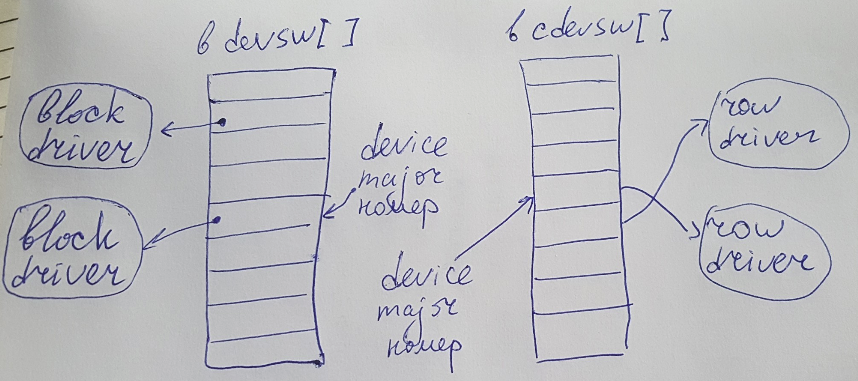
\includegraphics[width=\textwidth]{pic/1.png}
  \caption{pic}
\end{figure}

Важнейшая структура $device$. 

Структура $driver$ определяет точки входа драйвера и другую специфическую информацию. Разработчики драйверов должны знать состав этой структуры. Не все поля обязательно инициализировать.

\begin{lstlisting}[language=c]
//в сруктуру входят callback функции:
int (*probe);
int (*slave);
int (*cattach);
..
char *dev_name;
struct device **dev_list;
int (*dev_unattach)();
\end{lstlisting}